% Guardian-APC: conference paper draft (IEEE two-column format).
% Compile with: pdflatex guardian_apc && bibtex guardian_apc && pdflatex guardian_apc && pdflatex guardian_apc
% or upload this folder to Overleaf. Every number below comes from
% `modelforge_bench` (see ModelForge/research/results/results.json).
\documentclass[conference]{IEEEtran}
\usepackage{amsmath,amssymb,amsthm}
\usepackage{booktabs}
\usepackage{graphicx}
\usepackage{xcolor}
\usepackage{url}
\usepackage{pgfplots}
\pgfplotsset{compat=1.17}

\newtheorem{proposition}{Proposition}
\newtheorem{definition}{Definition}

\begin{document}

\title{Guardian-APC: Coverage-Guided Boundary Probing\\for Per-Pass Translation Validation in ML Compilers}

\author{\IEEEauthorblockN{Vaishnavi}
\IEEEauthorblockA{Department and institution (fill in)\\
Email (fill in)}}

\maketitle

\begin{abstract}
Machine-learning compilers rewrite computation graphs to make inference cheaper, and a single faulty rewrite can silently change predictions. Formal translation validation is precise but heavyweight; random differential testing is cheap but misses faults that only manifest near activation boundaries. We present \emph{Guardian-APC}, a lightweight per-pass validator built into the ModelForge model compiler. Guardian-APC (i)~uses interval bound propagation (IBP) to identify ReLU units whose kink is reachable on the input domain, (ii)~places probes exactly on each unstable kink \emph{at every depth} by Newton steps on the exact forward-mode input gradient, which is exact inside a linear region of a piecewise-linear network, and (iii)~schedules probes greedily by \emph{activation-pattern coverage} (APC), a monotone submodular objective whose greedy prefix is a $(1-1/e)$-approximation to the best fixed-budget coverage. Each rewrite is accepted only if every probe agrees with the graph before it; otherwise it is rolled back and a minimised, replayable counterexample is saved. In an equal-budget fault-injection study over 96 synthetic feed-forward models and 2{,}160 injected faults, Guardian-APC detects 99.1\% of observable faults with 128 probes, against 75.1\% for uniform random testing and 85.7\% for the previous Guardian design (paired exact McNemar $p<10^{-4}$ in both cases), needs 5.6 probes on average to first detection, and raises no false alarm on 96 negative controls. The result holds on held-out fault families (97.9\%), in deep layers (99.0\%), and under three further master seeds (99.2--99.5\%), at a synthesis cost of 3.5\,ms per model.
\end{abstract}

\begin{IEEEkeywords}
ML compilers, translation validation, differential testing, interval bound propagation, test prioritisation, coverage
\end{IEEEkeywords}

\section{Introduction}
Graph-level optimisation is central to ML compilers such as TVM~\cite{tvm} and Glow~\cite{glow}: operators are fused, constants folded and dead nodes removed. These rewrites are easy to get subtly wrong, and generated-network fuzzers such as NNSmith~\cite{nnsmith} have found many such bugs in production compilers. Formal approaches verify rewrite rules once and for all~\cite{tensorright} or validate each compilation with solvers~\cite{necula,pnueli,alive2}, but they need a formal semantics for every operator and can be expensive. At the other end, differential testing with random inputs is cheap and semantics-agnostic, yet it rarely lands where piecewise-linear networks are most fragile: near the kink of a ReLU.

This paper asks a narrow, testable question: \emph{for a fixed probe budget, can probes derived from the model's own activation boundaries detect faulty graph rewrites more often and earlier than random or generic probes?} We answer it with Guardian-APC, implemented in the open-source ModelForge compiler (C++17), and an equal-budget, paired, multi-model study.

\textbf{Contributions.}
\begin{enumerate}
\item \textbf{Deep boundary probing.} An IBP pre-pass selects unstable ReLU units; a Newton iteration on the exact forward-mode gradient places probes on each unit's kink at any depth and then at fixed pre-activation offsets on both sides (\S\ref{sec:boundary}).
\item \textbf{Activation-pattern coverage (APC) with an IBP-refined denominator}, and a greedy APC schedule with a $(1-1/e)$ prefix guarantee (\S\ref{sec:apc}).
\item \textbf{Per-pass guarded optimisation} with rollback, delta-debugging style witness minimisation and a JSON audit certificate (\S\ref{sec:guardian}).
\item \textbf{An open, reproducible benchmark}: a seeded model zoo, 11 fault families (5 held out from the probe design), a random oracle for observability, Wilson intervals and exact McNemar tests, plus a terminal studio and a web dashboard for inspection (\S\ref{sec:eval}).
\end{enumerate}

\section{Background and Related Work}
\textbf{Translation validation} checks each compiler run rather than the compiler~\cite{pnueli,necula}; Alive2 does so for LLVM IR with SMT~\cite{alive2}. TensorRight proves tensor rewrite rules correct for all shapes~\cite{tensorright}. Guardian-APC is deliberately weaker---a pass means ``no probe found a mismatch''---but needs only an executable reference semantics and runs in milliseconds.

\textbf{Compiler fuzzing.} Csmith~\cite{csmith} and NNSmith~\cite{nnsmith} \emph{generate programs or models} to find compiler bugs. We instead fix the model and \emph{generate inputs} that make a given rewrite's mistakes observable; the two are complementary.

\textbf{Neural coverage and verification.} Neuron coverage~\cite{deepxplore,deepgauge} has been criticised as a weak test-adequacy proxy for model robustness~\cite{harel}. We use coverage for a different purpose---scheduling inputs to expose \emph{compiler} faults---and refine its denominator with IBP~\cite{ibp}, a sound but loose bound also used in certified training. Complete verifiers such as Reluplex~\cite{reluplex} could replace IBP for tighter stability but at much higher cost.

\section{Approach}
\subsection{Setting}
A model is lowered to an SSA-style IR $G$ over Gemm, MatMul, Add, ReLU, Sigmoid and Softmax. An optimisation pass proposes $G'$. Given an input domain $D=[-r,r]^n$ (we use $r=10$) and a tolerance $\tau=10^{-5}$, a probe $x\in D$ \emph{exposes} the rewrite if $\|G(x)-G'(x)\|_\infty>\tau$ or $\arg\max G(x)\neq\arg\max G'(x)$. Guardian accepts $G'$ iff no probe in its suite $P$, $|P|\le B$, exposes it.

\subsection{Interval bound propagation}
We propagate boxes through the IR: interval products for Gemm/MatMul, sums for Add, monotone maps for ReLU and Sigmoid, and the bound $s_i\in[\,(1+\sum_{j\ne i}e^{u_j-l_i})^{-1},\,(1+\sum_{j\ne i}e^{l_j-u_i})^{-1}]$ for Softmax. Each ReLU unit with pre-activation bound $[l,u]$ is \emph{stable inactive} ($u\le 0$), \emph{stable active} ($l>0$) or \emph{unstable}. A liveness pass excludes activations that cannot reach the output, so no budget is spent on dead code.

\subsection{Deep boundary probes}\label{sec:boundary}
For an unstable unit $z_k(x)$ at any depth, we iterate
\begin{equation}
x_{t+1}=\Pi_D\!\left(x_t-\frac{z_k(x_t)}{\|\nabla z_k(x_t)\|^2}\nabla z_k(x_t)\right),
\end{equation}
where $\nabla z_k$ is computed exactly by forward-mode Jacobian propagation under the activation pattern of $x_t$, and $\Pi_D$ clips to $D$. We start from $0$ and, if the unit is locally dead, from up to three seeded random points.
\begin{proposition}
If $G$ is piecewise linear and $x_t$ and the Newton target lie in the same linear region inside $D$, then $z_k(x_{t+1})=0$.
\end{proposition}
\noindent\emph{Proof.} In that region $z_k(x)=w^\top x+b$ with $w=\nabla z_k(x_t)$, and substituting the update gives $w^\top x_t+b-z_k(x_t)=0$. \hfill$\square$

From the solved point we step to pre-activation targets $\{-0.05,\,5\!\cdot\!10^{-4},\,5\!\cdot\!10^{-3},\,5\!\cdot\!10^{-2}\}$ with one correction step each, so faults confined to bands of unknown width around the kink become observable. Units are chosen round-robin across layers (at most 64), so wide early layers do not starve deep ones.

\subsection{Activation-pattern coverage}\label{sec:apc}
\begin{definition}
Partition each unit's pre-activation into six bins: $(-\infty,-0.1)$, $[-0.1,0]$, $(0,10^{-3}]$, $(10^{-3},10^{-2}]$, $(10^{-2},10^{-1}]$, $(0.1,\infty)$. A (unit, bin) state is \emph{feasible} if the IBP interval meets the bin. The APC of a suite $P$ is the fraction of feasible states hit by some $x\in P$; \emph{boundary APC} restricts to the four bins around the kink.
\end{definition}
Coverage $C(P)$ is a union of state sets, hence monotone and submodular. Guardian orders the candidate pool (generic probes, first-layer affine probes, decision-boundary bisection probes and deep boundary probes) greedily by marginal coverage gain; probes that add nothing keep their original order. By the classic result for maximum coverage, every greedy prefix of length $B$ achieves at least $(1-1/e)$ of the best $B$-subset of the pool. This matters because Guardian's first-detection latency depends on order.

\subsection{Guarded optimisation}\label{sec:guardian}
Each pass (constant folding, Gemm+ReLU fusion, dead-node removal) runs on a copy. Guardian generates the APC-ordered suite from the graph \emph{before} the pass, compares outputs and predicted classes, and accepts or rolls back. On rejection it shrinks the first witness coordinate-wise toward zero while preserving the mismatch and writes it to \texttt{counterexample\_<pass>.json}; accepted decisions, probe count, maximum error and APC go into \texttt{optimization\_certificate.json}. Only the accepted graph is emitted as C++.

\section{Evaluation}\label{sec:eval}
\subsection{Setup}
\textbf{Corpus.} 96 He-initialised classifiers; depth cycles through 1--4 hidden ReLU layers (24 models each), widths 4--16, inputs 4--16, classes 2--5; each includes an output-unreachable ReLU. IBP labels 2{,}346 of 2{,}357 units unstable on $D$, so IBP rarely prunes on this domain.

\textbf{Faults.} Per activation layer: dead zones of width $10^{-1},10^{-2},10^{-3}$ (\emph{design aligned}: they match the probe offsets) and four \emph{held-out} or global families: a dead zone of log-uniform width in $[10^{-4},10^{-1}]$, an upper clamp at a random level in $[1,6]$ (a wrong ReLU6-style fusion), a leaky ReLU with slope $10^{-2}$ (wrong lowering) and ReLU$\to$Sigmoid. Per model: a $10^{-3}$ weight perturbation and a $10^{-2}$ bias perturbation (held out), a dropped bias, Softmax$\to$Sigmoid, and a rewrite of the unreachable node as negative control. In total 2{,}160 faults.

\textbf{Observability.} A fault is observable if any suite or a 4{,}000-probe uniform random oracle exposes it: 2{,}019 are observable, 45 unknown (excluded and reported), 96 are controls.

\textbf{Strategies} (all padded with uniform random probes to exactly $B$): uniform random on $D$ (5 seeds), \emph{generic} operator-aware probes, \emph{Guardian v1} (generic + first-layer affine probes + decision-boundary bisection), and Guardian-APC with three ablations: deep boundary probes only, v1$\cup$deep unordered, and APC order without deep probes. Statistics: Wilson 95\% intervals; exact two-sided McNemar tests on paired outcomes (random contributes one pair per seed).

\subsection{RQ1: Effectiveness at equal budget}
\begin{table}[t]
\centering
\caption{Detection of 2{,}019 observable faults at $B=128$ (master seed 20260917). ``1st'': mean probes to first detection among detected faults; APC: mean activation-pattern coverage per model.}
\label{tab:main}
\setlength{\tabcolsep}{3.5pt}
\begin{tabular}{lrrrrr}
\toprule
Strategy & Rate & 95\% CI & 1st & APC & ms \\
\midrule
Uniform random & 75.1 & [74.2, 75.9] & 11.0 & 51.0 & 0.01\\
Generic & 83.9 & [82.2, 85.4] & 9.4 & 64.5 & 0.02\\
Guardian v1 & 85.7 & [84.1, 87.1] & 11.2 & 67.4 & 0.09\\
\midrule
Deep boundary only & 98.1 & [97.4, 98.6] & 9.9 & 95.6 & 1.29\\
v1 $\cup$ deep, unordered & 94.4 & [93.3, 95.3] & 20.0 & 74.7 & 1.36\\
APC order, no deep & 85.8 & [84.2, 87.3] & 5.1 & 67.6 & 0.78\\
\textbf{Guardian-APC} & \textbf{99.1} & [98.6, 99.4] & 5.6 & \textbf{97.9} & 3.51\\
\bottomrule
\end{tabular}
\end{table}

Table~\ref{tab:main} shows that Guardian-APC detects 99.1\% of observable faults, 24.0 points above random and 13.4 above v1. Paired exact McNemar tests favour Guardian-APC over every baseline: 2{,}451 vs.\ 26 discordant pairs against random, 273 vs.\ 2 against v1, 311 vs.\ 4 against generic (all $p<10^{-4}$). No strategy flagged any of the 96 negative controls.

\subsection{RQ2: Efficiency across budgets}
\begin{figure}[t]
\centering
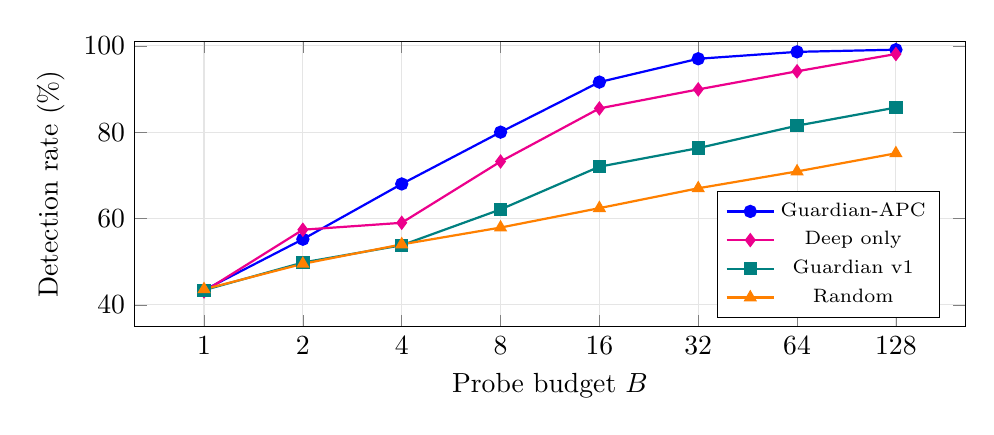
\begin{tikzpicture}
\begin{axis}[width=\columnwidth,height=5.2cm,xmode=log,log basis x=2,xtick={1,2,4,8,16,32,64,128},xticklabels={1,2,4,8,16,32,64,128},xlabel={Probe budget $B$},ylabel={Detection rate (\%)},ymin=35,ymax=101,legend pos=south east,legend style={font=\scriptsize},grid=major,grid style={gray!20}]
\addplot[thick,blue,mark=*] coordinates {(1,43.4)(2,55.2)(4,68.0)(8,80.0)(16,91.6)(32,97.0)(64,98.6)(128,99.1)};
\addplot[thick,magenta,mark=diamond*] coordinates {(1,43.1)(2,57.4)(4,59.0)(8,73.2)(16,85.5)(32,89.9)(64,94.1)(128,98.1)};
\addplot[thick,teal,mark=square*] coordinates {(1,43.4)(2,49.8)(4,53.8)(8,62.1)(16,72.0)(32,76.3)(64,81.5)(128,85.7)};
\addplot[thick,orange,mark=triangle*] coordinates {(1,43.6)(2,49.5)(4,54.0)(8,57.9)(16,62.4)(32,67.0)(64,70.9)(128,75.1)};
\legend{Guardian-APC, Deep only, Guardian v1, Random}
\end{axis}
\end{tikzpicture}
\caption{Share of observable faults exposed within the first $B$ probes of each 128-probe suite.}
\label{fig:curve}
\end{figure}

Fig.~\ref{fig:curve} plots detection within the first $B$ probes. Guardian-APC reaches 91.6\% at $B=16$, where random reaches 62.4\% and v1 72.0\%. Counting misses as $B{+}1$, its mean probes to detection is 6.7 versus 40.4 for random and 28.1 for v1. Re-running the whole study with a 32-probe budget gives 97.2\% for Guardian-APC, 67.1\% for random and 76.5\% for v1.

\subsection{RQ3: Ablation}
Deep boundary probes are the main source of detection power (98.1\% alone), but they need the right order: appended after v1's probes and truncated at $B=128$, the unordered union detects only 94.4\%, and at $B=32$ it collapses to v1's 76.5\% because no deep probe survives truncation. APC ordering without deep probes lowers latency (5.1 probes) but cannot raise the ceiling (85.8\%). Their combination dominates both; against deep-only it wins 22 vs.\ 2 discordant pairs ($p<10^{-4}$).

\subsection{RQ4: Generalisation}
Narrow dead zones separate the strategies most: for width $10^{-3}$ Guardian-APC detects 240/240, v1 27.5\%, generic 17.9\% and random 4.5\%. On held-out families Guardian-APC detects 97.9\% (random 85.4\%, v1 90.9\%); on the held-out random-width dead zone, 94.0\% (random 39.1\%, v1 64.7\%). Faults beyond the first activation layer, where v1 has no model-conditioned probes, are detected at 99.0\% (v1 82.1\%). Guardian-APC is \emph{not} better everywhere: on the $10^{-3}$ weight perturbation it matches v1 (94.5\%) and is below random (97.1\%), because broad random sampling already exercises the perturbed weight's input coordinate.

\textbf{Seed robustness.} With master seeds 1, 2 and 3 (new models, faults and random baselines) Guardian-APC detects 99.4\%, 99.5\% and 99.2\%, random 75.4\%, 74.8\% and 73.7\%, and v1 85.7\%, 86.1\% and 86.4\%; comparisons against random, generic and v1 remain significant at $p<10^{-4}$, and against deep-only at $p\le 5\times10^{-4}$.

\subsection{RQ5: Cost}
Probe synthesis (IBP, Newton solving and greedy ordering) takes 3.5\,ms per model on average on one core (GCC 13.3, Linux); the complete 96-model study, including every fault and baseline, finishes in 3.3\,s. Within the compiler, Guardian checks a pass on the Iris demo model with 85 probes in under a millisecond.

\section{Threats to Validity}
\textbf{Synthetic models.} Models are small dense networks (widths $\le16$); convolutions, attention and real ONNX models are future work. \textbf{Fault realism.} Dead-zone widths partly match the probe offsets; we therefore report held-out families separately. \textbf{Loose bounds.} On $D=[-10,10]^n$, IBP marks almost all units unstable and proves no fault unobservable; tighter bounds (e.g.\ linear relaxations) would prune more. \textbf{Oracle.} Observability uses the union of all suites plus a random oracle, so faults no method finds are labelled unknown, not missed. \textbf{Common-mode errors.} The interpreter and code generator share operator definitions; an independent runtime check (e.g.\ ONNX Runtime) is supported but not part of this study. \textbf{Not a proof.} Passing Guardian is evidence, not formal equivalence.

\section{Conclusion}
Placing probes on the model's own activation kinks at every depth, and ordering them by activation-pattern coverage, turns per-pass differential testing into a strong, cheap guard for ML compiler rewrites: 99.1\% detection at 128 probes, 91.6\% at 16, no false alarms, and a replayable counterexample whenever a rewrite is rolled back. The implementation, benchmark, terminal studio and dashboard are open source and regenerate every number in this paper with one command.

\section*{Reproducibility}
\texttt{cmake -S . -B build \&\& cmake --build build --config Release}, then \texttt{modelforge\_bench} (add \texttt{--seed}, \texttt{--budget}, \texttt{--models}). It writes \texttt{results.json}, per-case \texttt{cases.csv} and the dashboard data file.

\bibliographystyle{IEEEtran}
\bibliography{references}

\end{document}
